\chapter{测试}
\label{测试}
\defaultfont

软件测试是指基于一组有限的测试用例(通常是从无限的执行域中进行适当选择),动态地验证程序的行为,并于预期行为进行对比\cite{.software}。常见的测试方法有白盒测试和黑盒测试,白盒测试是基于代码的测试,一般用于单元测试,由程序员进行测试;黑盒测试基于需求描述,通常用于功能测试,一般由测试人员进行。白盒测试在系统开发过程中已经完成,下面记录了功能测试。

\section{系统测试环境}

如表\ref{test-system}所示。

\begin{table}[htbp]
  \centering
  \song\wuhao
  \caption{系统配置表}
  \label{test-system}
\begin{tabular}{lll}
\hline
\multicolumn{3}{c}{硬件配置}                                                                 \\ \hline
\multirow{4}{*}{服务器端} & CPU    & Intel(R) Core(TM) i7-7700HQ CPU @ 2.80GHz               \\
                      & 内存     & 6GB                                                     \\
                      & 硬盘     & 1TB                                                     \\
                      & 网卡     & 1000M以太网卡                                               \\ \hline
\multirow{4}{*}{客户端}  & CPU    & Intel(R) Core(TM) i7-7700HQ CPU @ 2.80GHz               \\
                      & 内存     & 10GB                                                    \\
                      & 硬盘     & 1TB                                                     \\
                      & 网卡     & 1000M以太网卡                                               \\ \hline
\multicolumn{3}{c}{软件配置}                                                                 \\ \hline
\multirow{2}{*}{服务器端} & 操作系统   & Ubuntu 20.04.2 LTS                                      \\
                      & 数据库服务器 & 8.0.23-0ubuntu0.20.04.1 for Linux on x86\_64 ((Ubuntu)) \\ \hline
\multirow{2}{*}{客户端}  & 操作系统   & Windows 10 家庭中文版(版本号20H2)                               \\
                      & 浏览器    & Microsoft Edge(版本90.0.818.62)                           \\ \hline
\end{tabular}
\end{table}

\section{测试用例与测试过程}

\begin{table}[htbp]
  \centering
  \song\wuhao
  \caption{ 测试用例表 }
  \label{test-usecase-table}
\begin{tabular}{lll}
\hline
测试项目   & 测试用例                  & 测试结果   \\ \hline
用户登录   & 验证不同用户是否能正确登录         & 功能准确实现 \\
论文上传   & 验证能否正确上传pdf论文         & 功能准确实现 \\
论文下载   & 验证能否正确下载pdf论文         & 功能准确实现 \\
论文更新   & 验证能否正确更新选定的论文         & 功能准确实现 \\
论文评论   & 验证能否正确新建评论,回复评论       & 功能准确实现 \\
问题标签   & 验证能否正确为评论添加标签         & 功能准确实现 \\
论文评分   & 验证能否正确为所选论文评分         & 功能准确实现 \\
论文得分统计 & 验证能否正确统计论文的得分情况       & 功能准确实现 \\
教师任务统计 & 验证能否正确统计教师的评审评分任务完成情况 & 功能准确实现 \\
学生管理   & 验证能否正确修改学生信息          & 功能准确实现 \\
教师管理   & 验证能否正确修改教师信息          & 功能准确实现 \\ \hline
\end{tabular}
\end{table}

用户登录测试如图\ref{login-test},需要测试不同用户的登录能够成功,一点是用户只有输入正确的用户名和密码才能正确登录,另一点是用户只有选择正确的用户类型才能正确登录。每类用户都需要进行多次测试,使用正确用户名,错误用户名,正确密码,错误密码,正确类型,错误类型,各自组合测试。

\begin{figure}[htbp]
  \centering
  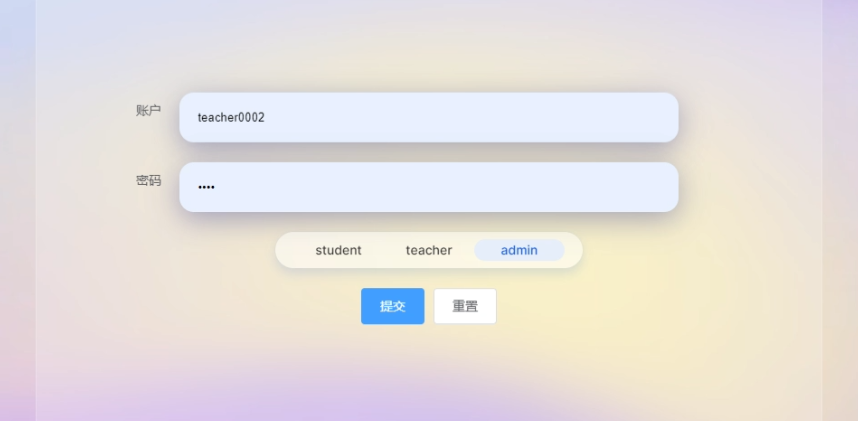
\includegraphics[scale = 0.57]{out/figure/测试/login-test.png}
  \caption{\song\wuhao 登录测试图}
  \label{login-test}
\end{figure}

论文上传测试如图\ref{upload-test}所示,需要测试学生上传的论文能否正确的使用后台保存到后台的数据库,论文的所属学生是否是登录用户。

\begin{figure}[htbp]
  \centering
  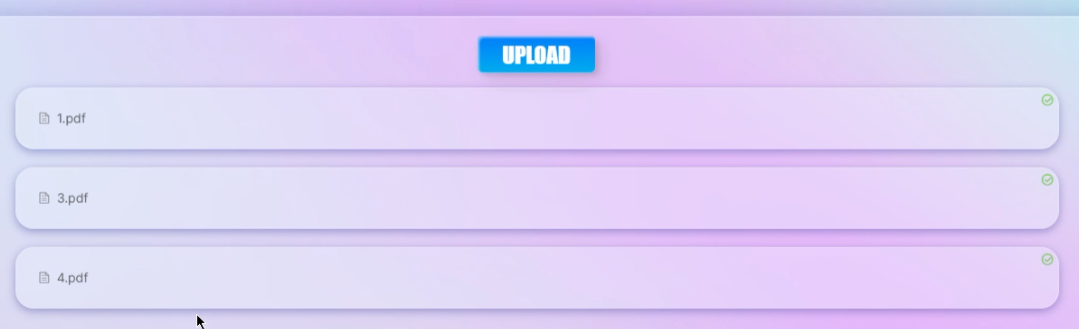
\includegraphics[scale = 0.5]{out/figure/测试/upload-test.png}
  \caption{\song\wuhao 论文上传测试图}
  \label{upload-test}
\end{figure}

论文下载测试如图\ref{download-student-test}和图\ref{download-teacher-test}所示,需要在学生页面和教师页面都测试,需要测试点击下载按钮能否下载文件,下载的文件能否正常打开,文件的内容是否正确。

\begin{figure}[htbp]
  \centering
  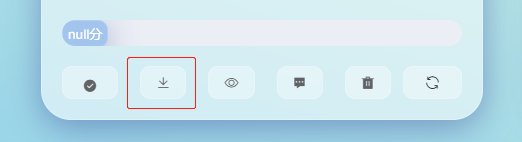
\includegraphics[scale = 0.6]{out/figure/测试/download-student-test.png}
  \caption{\song\wuhao 学生论文下载测试图}
  \label{download-student-test}
\end{figure}

\begin{figure}[htbp]
  \centering
  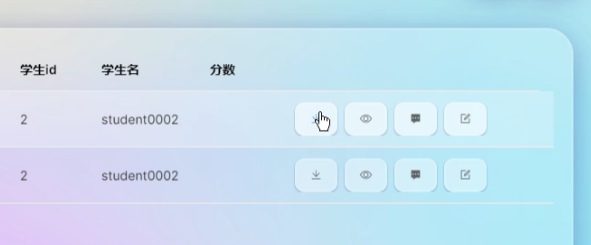
\includegraphics[scale = 0.6]{out/figure/测试/download-teacher-test.png}
  \caption{\song\wuhao 教师论文下载测试图}
  \label{download-teacher-test}
\end{figure}

论文更新模块测试如图\ref{file-refresh-test}所示,学生点击更新论文按钮,选择新的文件,点击确定,文件上传。需要测试文件是否更新成功,数据库中的文件附加信息(文件名,文件类型,所属学生等)是否正确,更新的文件能否下载,下载的文件及其附加信息是否正确。

\begin{figure}[htbp]
  \centering
  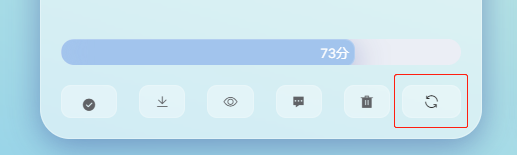
\includegraphics[scale = 0.6]{out/figure/测试/file-refresh-test.png}
  \caption{\song\wuhao 更新文件测试图}
  \label{file-refresh-test}
\end{figure}

论文评论模块测试如图\ref{comment-add},图\ref{comment-replay}所示,学生或教师可以新建评论(不点击回复按钮或者点击回复按钮之后点击取消),测试新建评论是否是顶级评论,点击评论条目右下角的回复(replay)按钮将选择回复这一条评论,需要测试回复的评论是否为选择的评论的子级,评论人是否为登录用户,刷新后评论条目结构是否正确,使用其他用户登录查看此论文评论是否一致。

\begin{figure}
  \centering
  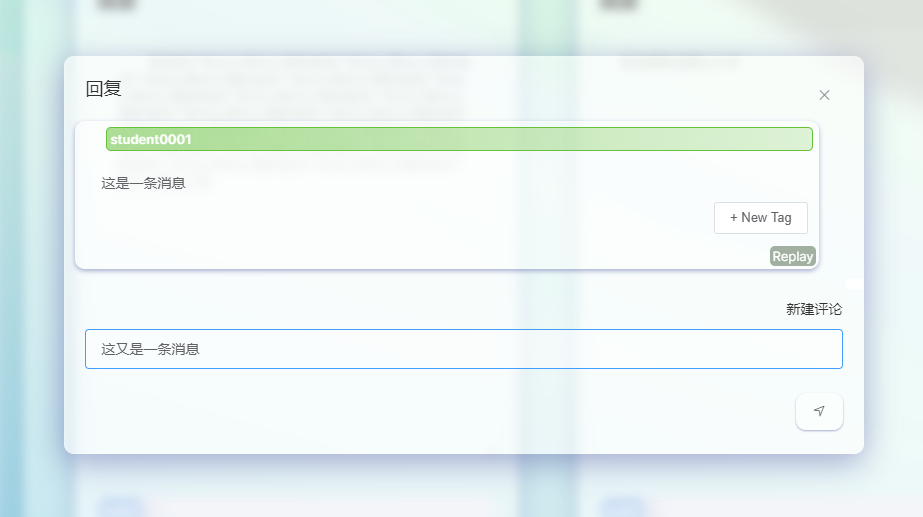
\includegraphics[scale = 0.6]{out/figure/测试/comment-add.png}
  \caption{\song\wuhao 新建评论测试图}
  \label{comment-add}
\end{figure}

\begin{figure}
  \centering
  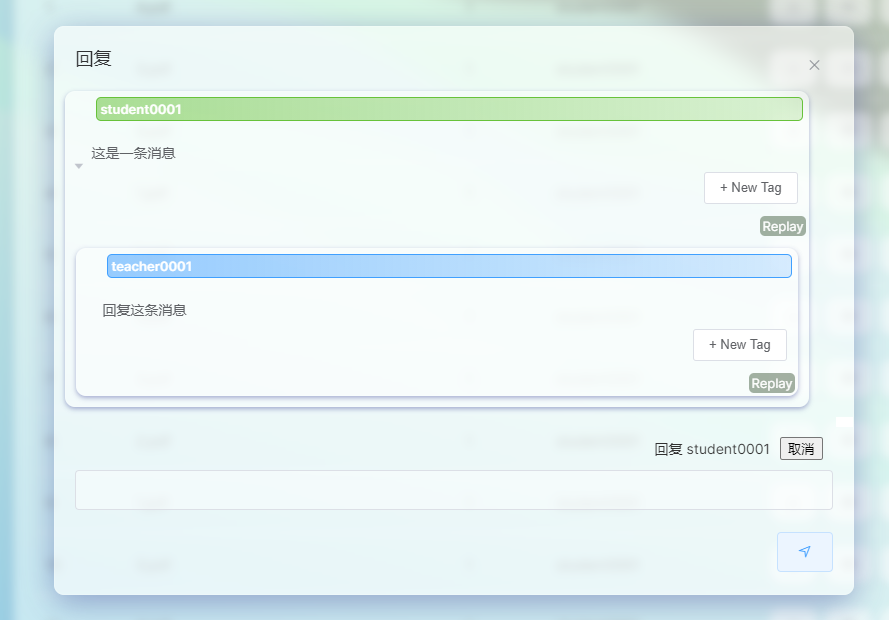
\includegraphics[scale = 0.6]{out/figure/测试/comment-replay.png}
  \caption{\song\wuhao 回复评论测试图}
  \label{comment-replay}
\end{figure}

论文评分模块测试如图\ref{score-student}和图\ref{score-teacher}所示,教师可以点击评分按钮,弹出评分对话框,滑动分数滑动条可以选择分数,点击确定为学生评分。该部分需要测试是否可以评分,是否为正确的论文评分,分数是否正确,评分人是否正确记录,学生端是否正确显示分数。

\begin{figure}[htbp]
  \centering
  
\includegraphics[scale = 0.6]{out/figure/测试/score-student.png}
  \caption{\song\wuhao 学生查看得分测试图}
  \label{score-student}
\end{figure}

\begin{figure}[htbp]
  \centering
  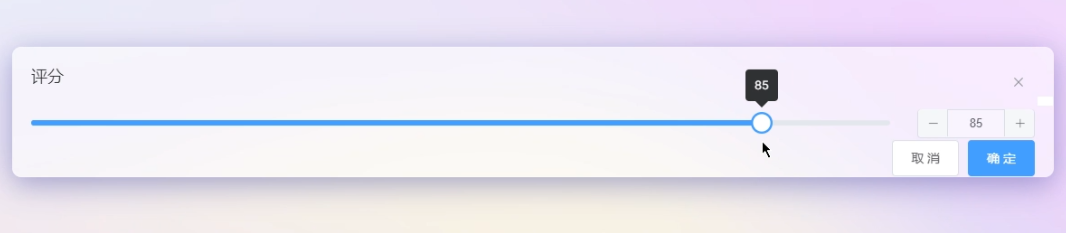
\includegraphics[scale = 0.6]{out/figure/测试/score-teacher.png}
  \caption{\song\wuhao 教师评分测试图}
  \label{score-teacher}
\end{figure}

论文得分统计模块测试如图\ref{statistic-score-student-test}所示,管理员可以切换论文得分统计页面,页面将展示学生的得分情况,需要测试各个分数段的人数是否正确,多次增删论文并评分,测试得分统计是否一致。

\begin{figure}[htbp]
  \centering
  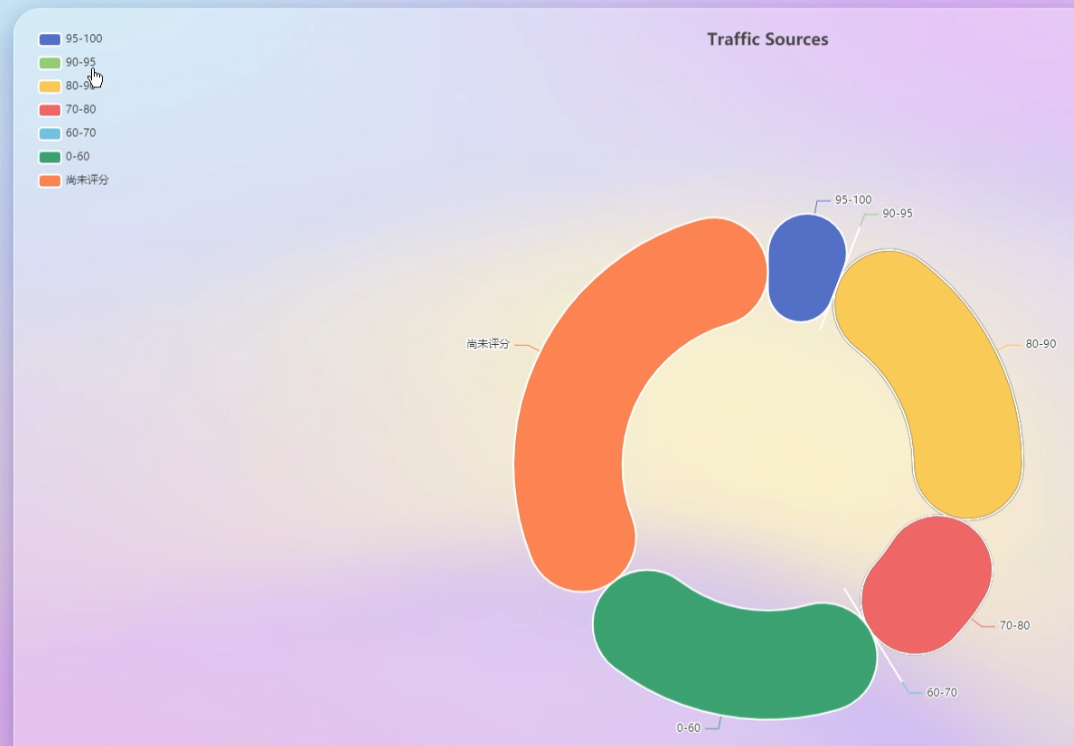
\includegraphics[scale = 0.48]{out/figure/测试/statistic-score-student-test.png}
  \caption{\song\wuhao 论文得分统计测试图}
  \label{statistic-score-student-test}
\end{figure}

教师评审任务完成情况统计模块测试如图\ref{statistic-teacher-task-test}所示,管理员可以切换到教师评审任务统计完成情况统计页面,需要测试各个教师管理的学生数是否正确,需要管理的所有论文数量是否正确,已经评分的论文数量是否正确,尚未评分的论文数量是否正确。

\begin{figure}[htbp]
  \centering
  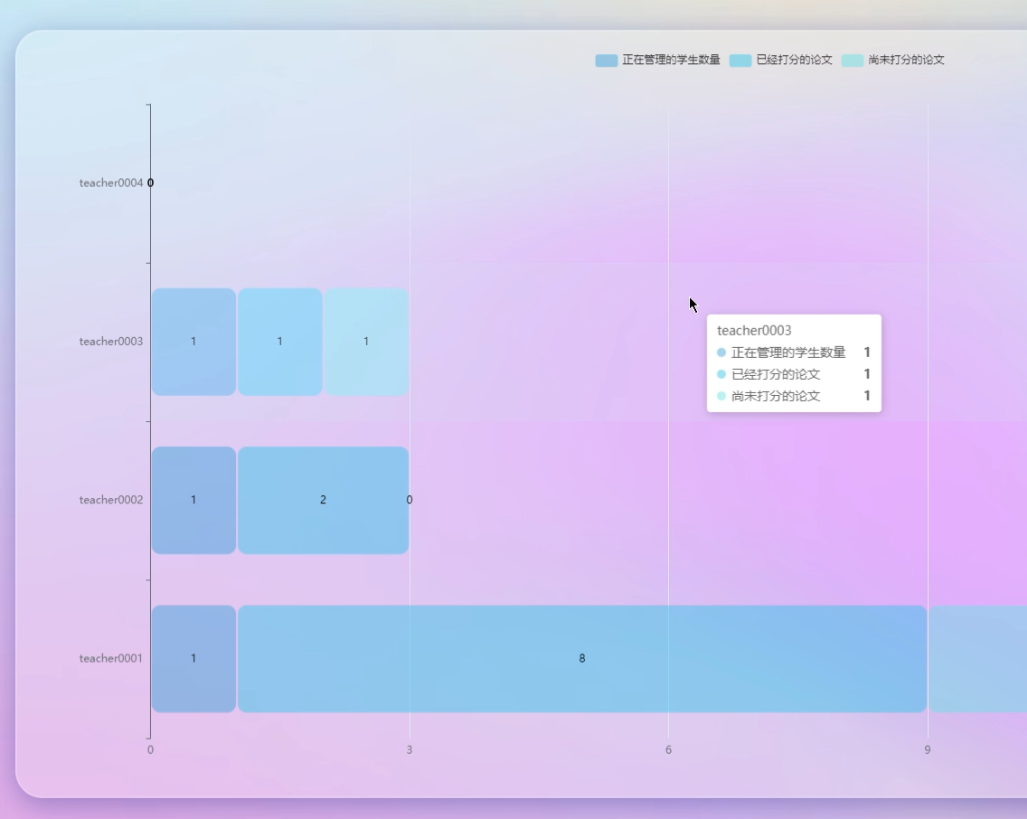
\includegraphics[scale = 0.48]{out/figure/测试/statistic-teacher-task-test.png}
  \caption{\song\wuhao 教师任务统计测试图}
  \label{statistic-teacher-task-test}
\end{figure}

人员管理模块测试如图\ref{manage-students}和图\ref{manage-edit-student-test}所示,在查看方面,需要测试所有学生信息是否正确显示;在修改信息方面需要测试各个字段的更改是否有效,密码不更改是否会清空密码,修改密码后是否能使用新密码登录。

\begin{figure}
  \centering
  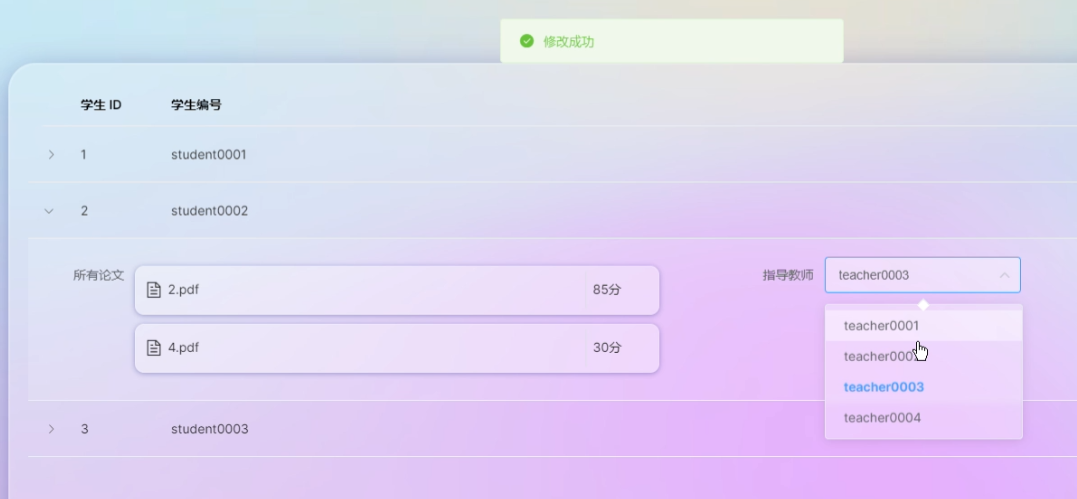
\includegraphics[scale = 0.6]{out/figure/测试/manage-students.png}
  \caption{\song\wuhao 学生管理功能测试}
  \label{manage-students}
\end{figure}

\begin{figure}[htbp]
  \centering
  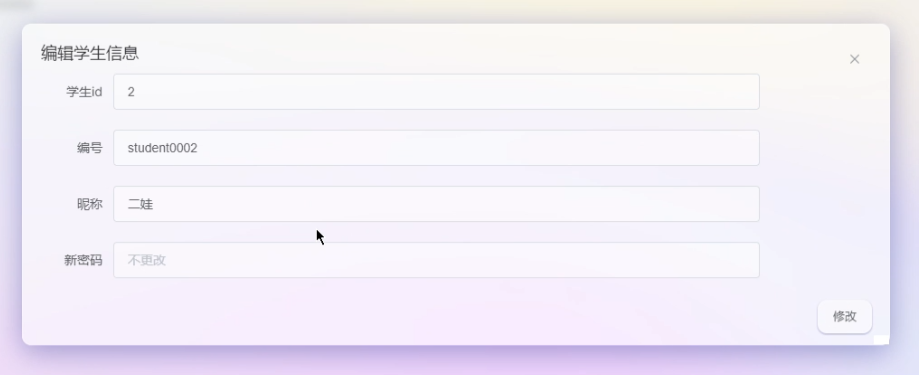
\includegraphics[scale = 0.6]{out/figure/测试/manage-edit-student-test.png}
  \caption{\song\wuhao 编辑学生功能测试}
  \label{manage-edit-student-test}
\end{figure}

\section{本章小结}

本章介绍了测试的过程以及测试结果,出现的问题都已解决,程序可正确运行。